\chapter{Implementierung}\label{ch:Implementierung}

Aus den bis hier beschriebenen Anforderungen für die Ausführung der Experimente ergibt sich die Notwendigkeit einer eigenen Software Lösung. Existierende Lösungsansätze müssen gegen verschiedene Benchmarks ausgeführt und evaluiert werden - geleitet von einer zentralen Platform, einen Orchestrator. Zu diesem Zweck habe ich\todo{"ich"? wie formuliert man das?} das Tool ''EvaluationPlatform'' gebaut. Dieses ist offen zugänglich und kann auf GitHub\footnote{https://github.com/Tim-Dietrich/EvaluationPlatform} gefunden werden. Dieses Kapitel beschreibt im weiteren die zugrunde liegenden Entscheidungen, die beim entwickeln der Anwendung getroffen wurden und wie diese implementiert wurde. 

\section{Wahl des Tech-Stacks}\label{ch:Wahl des Tech-Stacks}

% Diese Sektion beschreibt die Anwendung, welche gebaut wurde um die Fragen \rqref{RQ1} und \rqref{RQ2} transparent und möglichst gerecht beantworten zu können. Dabei wird erklärt wie diese Anwendung sturkturiert wurde und welche Entscheidungen dafür getroffen wurden.

\todo[inline]{Info: ''Ziel der Anwendung'' gehört hier nicht hin, das ist Konzept/Anforderungen. Die Obligationen wurden nach NFA verschoben.}
% \subsubsection{Ziel der Anwendung}\label{ch:Ziel der Anwendung}

% Wie bereits in \todo{ref to Oben, Struktur Idee etc.} beschrieben wurde, sollen in dieser Arbeit bestehende Lösungsansätze verglichen werden. Dies passiert wie in \todo{ref to Benchmarks} beschrieben via Benchmarks, welche genutzt werden um jeden Lösungsansatz unter gleichen Bedienungen zu testen. Zu diesem Zweck bedarf es einer Anwendung welche diesen Ablauf gewährleisten kann. Diese Platform unterliegt im Grunde 4 verschiedenen Obligationen:

% \begin{enumerate}
%     \item Generierter Code muss unabhängig und isoliert von seiner Umgebung laufen können. Das selbe gillt für das Grading
%     \item Der laufende Benchmark bewertet die Ergebnisse einer laufenden Code-Generierungsanwendung. Die Bewertung wird einzig und allein vom Benchmark definiert.
%     \item Alle Code-Generierungsanwendungen müssen austauschbar sein. Dafür dürfen weder der Benchmark noch andere funktionale Aspekte der Anwendung verändert werden.
%     \item Jeder Durchlauf eines Experiments muss vollständig nachvollziehbar sein. Versionen, Modelle und Parameter müssen auch nach durchführung ersichtlich sein.
% \end{enumerate}

% \todo[inline]{Erklären welche Parameter wir fest halten und welche evtl. variabel sein könne, siehe Prof. Both Konsultation \#6}

% Der Umfang dieser Anwendung wird bewusst schmal gehalten. Zweck ist lediglich das orchestrieren von Experimenten unter den bereits genannten Gesichtspunkten. Damit existiert eine klare Abgrenzung zu anderen Platformen, wie z.B. ''Bestenlisten'' oder ''Agent-Frameworks''.

% \subsubsection{Wahl eines Frameworks}

Der Umfang dieser Arbeit ist lediglich die Evaluation bestehender Lösungen. Somit ist es ziehlführend, bereits existierende Lösungen / Frameworks für die Nutzung eines Orchestrators einzubinden, anstatt diesen selbst zu kreieren. Eine solche bestehende Plattform erlaubt es den Fokus dieser Arbeit auf die Evaluation von existierenden Lösungen zu legen, anstatt zuerst selbst eine Plattform erstellen zu müssen.

Um die Wahl einer Orchestrierungsplatform zu begründen wurde ein explorativer Machbarkeitsversuch durchgeführt. Dieser Bestand aus dem Ziel, die Plattform aufzusetzen und einen einfachen Task zu starten. Der Task war hier lediglich das generieren eines lauffähigen Taschenrechners mit minimalen Funktionen. 

Es ist relevant hier zu erwähnen dass die Evaluation pur explorativ war und nicht systematischer Natur. Weiterhin wurde diese Exploration durch die Nutzung von LLM basierten Agenten umgesetzt. Die Wahl der zu nutzenden Plattform ist daher eher als Mittel zum Zweck zu sehen, nicht als Ergebnis dieser Arbeit.

Die Evaluation der Plattformen erfolgte gegenüber den Anforderungen, welche in den Sektionen \ref{ch:Funktionale Anforderungen} sowie \ref{ch:Nich-Funktionale Anforderungen} definiert wurden. Die betrachteten Plattformen wurden durch händische Suche gefunden.

Es ergaben sich daraus folgende Evaluierungen:

\begin{enumerate}
    \item \textbf{Eigene Plattform} \\ Wie bereits beschrieben, ist das Entwickeln einer eigenen Plattform nicht im Rahmen dieser Arbeit. Der Aufwand gegenüber allen Anforderungen wäre eine komplette Selbst-Entwicklung, was hier nicht tragfähig ist. Somit scheidet diese Option faktisch aus.
    \item \textbf{Benchmark-spezifische Skripte} \\ Die betrachteten Benchmarks (z.B. NL2Repo-Bench, SWE-Pro) kommen jeweils mit eigenen Skripten, um deren Ausführung zu ermöglichen. Dies funktioniert prinzipiell, erfordert aber ähnlich zur eigenen Plattform maßgeblichen Entwicklungsaufwand. Ferner ist durch die unterschiedlichen Implementierungen keine Vergleichbarkeit unter den verschiedenen Benchmarks gegeben. Aus diesem Grund wurde diese Option nicht weiter evaluiert.
    \item \textbf{Inspect AI} \\ TODO nachtragen
    \item \textbf{Harbor} \\ TODO nachtragen
\end{enumerate}

Nach Ablauf dieser Evaluation wurde sich für Harbor als zugrunde liegende Plattform entschieden. Neben der relativ einfachen Implementierung, deckt dieses Framework auch am besten die gegebenen Anforderungen ab. Wie bereits erwähnt, ist allerdings auch Harbor nicht in der Lage, alle Anforderungen ohne einen eigenen Entwicklungsaufwand zu erfüllen. 

\todo[inline, color=red]{Anforderungs-ID's sind doch notwendig! nachholen!}

\section{Architektur der Evaluierungsplatform}\label{ch:Architektur der Evaluierungsplatform}

Diese Sektion stellt die tatsächliche Implementierung der Evaluierungsplattform dar. Zum besseren Verständniss wurde die Architektur in 2 Einzelteile aufgeteilt:

\begin{enumerate}
    \item Das initiale Setup für den Orchestrator
    \item Die Architektur einer tatsächlichen Durchführung
\end{enumerate}

Hierbei gilt zu unterscheiden woher die verschiedenen Komponenten stammen. Zu diesem Zweck dient zunächst eine farbliche Legende, diese ist in der Figur \ref{fig:legend} zu erkennen.

\begin{figure}[H]
    \centering
    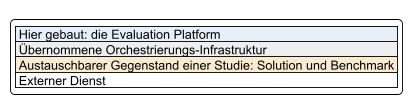
\includegraphics[width=0.75\linewidth]{evaluation_legend.png}
    \caption{Enter Caption}
    \label{fig:legend}
\end{figure}

Wir bereits in den Anforderungen beschrieben\todo{ref zur ID}, benötigt die Evaluierung zwingend eine feste einheitliche Definition aller Experimente. Bevor ein Durchlauf auf den tatsächlichen Integrator (hier Harbor) zugreift, muss also die Definition des Experimentes validiert und aufgelöst werden. Dieser Prozess ist in Figur \ref{fig:setup} zu sehen.

\begin{figure}[H]
    \centering
    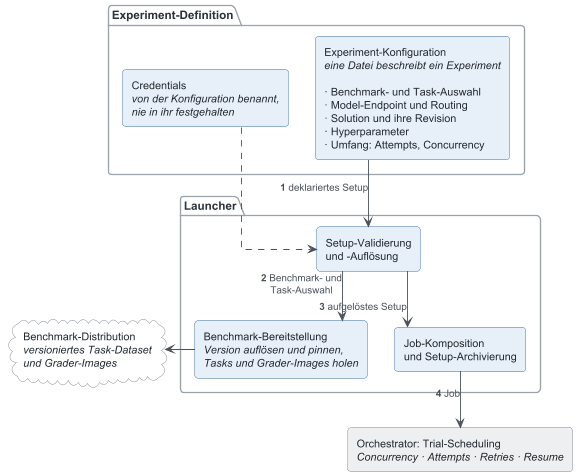
\includegraphics[width=1\linewidth]{evaluation_setup.png}
    \caption{Enter Caption}
    \label{fig:setup}
\end{figure}

\todo[inline, color=red]{WARNUNG: TEXT AUS ALTEM KAPITEL ÜBERNOMMEN; FÜR DIESE SEKTION ANPASSEN!}

Mit Harbor haben wir ein bestehendes Framework welches die Integration von verschiedenen Benchmarks durch seine eigene Dataset registry erlaubt. Währe das Ziel unserer Experimente die Evaluation von nativen Agenten/LLM-Integrationen würde dies für die weitere Durchführung genügen. Allerdings ergeben sich im Kontext dieser Arbeit 2 notwendige Änderungen:

\begin{enumerate}
    \item Das Ziel ist das Testen von Code-Generierungsanwendungen. Diese arbeiten nicht nach genormten Verfahren, jede Lösung ist individuell.
    \item Nicht \textit{alle} Benchmarks können nativ durch Harbor abgedeckt werden. Insbesondere NL2RepoBench\todo{cite} benötigt eine Anpassung, da den Entwicklern ein Fehler beim aufsetzen des Docker Images unterlaufen ist.
\end{enumerate}

Um diese Probleme zu beheben werden für alle integrierten Code-Generierungsanwendungen Integrationen geschrieben. Weiterhin existiert eine besondere Integration für NL2RepoBench, die dafür sorgt dass das benötigte Image über eine öffentlich zugängliche Platform bezogen wird. Die Integration für die einzelnen Code-Generierungsanwendungen wird in den jeweiligen Kapitel beschrieben um eine höhrere Transparenz zu gewährleisten. Fundamental dabei ist es, dass die Logik besagter Lösungen \textbf{nicht} angepasst wurde. Gemachte Modifikationen dieser Repositories zielen lediglich auf eine mögliche Integration ab, z.B. die Integration von Umgebungsvariablen via DotEnv\todo{evtl cite} Dateien.

\todo[inline]{Schlussendliche Erklärung der gewählten Architektur}

\begin{figure}[H]
    \centering
    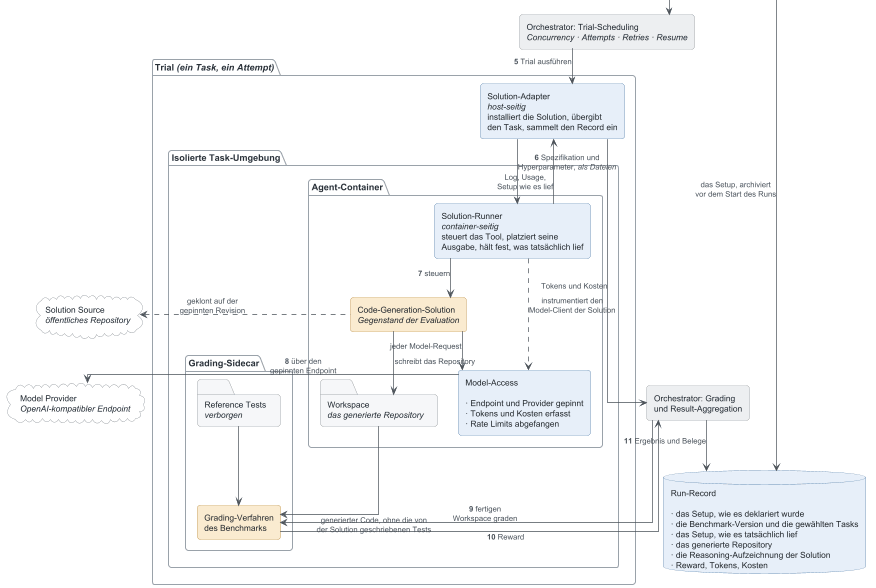
\includegraphics[width=1\linewidth]{evaluation_run.png}
    \caption{TODO: das passt von der größe nicht. Irgendwie was anderes ausdenken.}
    \label{fig:full_run}
\end{figure}

\section{Integration der Code-Generierungsanwendungen}\label{ch:Integration der Code-Generierungsanwendungen}

Wie bereits beschrieben lassen sich bestehende Code-Generierungsanwendungen nicht ohne weiteres in die Anwendung integrieren. Zwar haben einzelne Anwendungen wie \cite{dongSelfCollaborationCodeGeneration2024} bereits funktionierende Integrationen für Benchmarks, so ist es mit diesen aber nicht möglich eine uniforme Durchführung von Experimenten zu gewährleisten.

Demnach bedarf es für jede Anwendung einer Integration in den Harbor Workflow. Zuerst können damit folgende Kriterien sichergestellt werden:

\begin{enumerate}
    \item Freie Modelauswahl 
    \item Hyperparameter sind konfigurierbar
    \item Anwendungs-spezifische Parameter sind konfigurierbar
\end{enumerate}

Die Konfiguration dieser Werte erfolgt in der Evaluierungs-Platform und wird lediglich an die einzelnen Code-Generierungsanwendungen weitergereicht. Dabei unterstützen die einzelnen Konfigurationsdateien alle einzigartigen Parameter. Im folgenden ergeben sich daraus folgende Integrationen:

\todo[inline]{Integrationen für die einzelnen Anwendungen auf-listen mit ihren spezifischen Anforderungen.}

\subsection{Code-Team}

bla bla und so weiter mit subsections

\section{Implementierung der Referenz-Ansätze}

Die Sektion \ref{ch:Untersuchungsdesign} formuliert neben der Untersuchung bestehender Arbeiten auch die Inklusion von Referenzwerten durch zwei weitere Systeme (Single-Shot Basline \& Agentisches Verfahren). Im Gegensatz zu der Sektion \ref{ch:Integration der Code-Generierungsanwendungen} handelt es sich bei diesen Ansätzen nur bedingt um Integrationen, weswegen diese hier getrennt betrachtat werden.

\subsection{Single-Shot Baseline}\label{ch:Impl:Single-Shot Baseline}

Als Baseline im Vergleich dieser Arbeit dient ein Single-Shot-Ansatz. Die Implementierung dieses Ansatzes ist wie folgt geschehen:

\begin{enumerate}
    \item \textbf{Setup} \\ Initial werden analog zu anderen Ansätzen die Parameter der gegebenen Konfiguration bezogen.
    \item \textbf{Prompt-Erstellung} \\ Nach dem initialen Setup erfolgt die Erstellung des fertigen Prompts. Das Design dieses Prompts ist wichtig, denn er darf keine Lösungsstrategie angeben. Der hier genutzte Prompt \autoref{lst:prompt-singleshot} erklärt lediglich die vom Parser erwartete Ausgabestruktur, ohne die eine weitere Auswertung durch Harbor nicht möglich wäre. Die Anforderungen definieren weiterhin ''Zero-Shot'', weshalb keine Beispiele an den Prompt angehangen werden.
    \item \textbf{Ausführung} \\ Die vollständige Beschreibung der Aufgabe sowie der gegebene Prompt werden an das konfigurierte Modell übergeben.
    \item \textbf{Parsing} \\ Nach Antwort des Modells werden die Ergebnisse geparsed. Sollte die Antwort der erwarteten Struktur entsprechen, wird sie in einzelne Datein aufgeteilt und für die Evaluation im \texttt{workspace} Verzeichnis abgelegt.
\end{enumerate}

Nach diesem Ablauf erfolgt die gewohnte Evaluierung des Benchmarks, welcher durch das Harbor Framework orchestriert wird.

\subsection{Agentisches Verfahren}\label{ch:Impl:Agentisches Verfahren}

Das zweite Verfahren, welches als Refernz dient, ist das agentische Verfahren. Bei der Implementierung wurde keine explorative Suche oder eine Studie in betracht gezogen um ein Agenten-System auszuwählen. Da die Schaffung eigener Systeme prinzipiell nicht im Rahmen dieser Arbeit ist, wurde hier das bereits von Harbor bereitgestellte Agenten-System Terminus-2 \cite{Terminus2} gewählt.

Durch die bereits existierend Integration in den Harbor Workflow bedarf es hier keiner klassischen Integration wie bei bereits genannten Verfahren, allerdings mussten trotzdem kleine Anpassungen erfolgen:

\begin{enumerate}
    \item Die Vermittlung von Credentials erfolgt im Projekt durch eine speziell dafür geschaffene Überbrückung.
    \item Hyperparameter sind prinzipiell gleich; allerdings stellt Terminus-2 als Agenten-System einen extra Parameter \texttt{max\_turns} bereit, welcher hier gesondert konfiguriert werden muss. Dieser Parameter definiert die maximale Menge an Schritten des Agenten, was später für die Vergleichbarkeit wichtig wird.
\end{enumerate}

Das Verhalten des Agenten ist in dieser Implementierung nicht weiter beeinflußt.

\subsubsection{Terminus-2}

Ferner soll der von Harbor bereitgestellte Agent Terminus-2 hier kurz erklärt werden. Das Augenmerk liegt auf dessen Fähigkeiten und Eigenschaften, entnommen von \cite{Terminus2}:

\begin{itemize}
    \item Terminus-2 ist eine Implementiernug eines Agenten, gedacht zur Evlauation von LLMs bei deren Arbeit in Kommandozeilen Umgebungen.
    \item Es nutzt einen selbst betietelten ''single-tool approach'', durch welchen es in der Lage ist Tastenanschläge zu simulieren, Umgebungen zu navigieren, durch Output zu scrollen, Shells zu starten und mit Kommandozeilen-basierten Anwendungen zu interagieren.
    \item Die Ausführung der Logik läuft in einem sepparatem Python Prozess, welcher durch eine Docker-basierte Ausführung sicher und isoliert arbeitet. Der Agent hat somit nur Zugriff auf gegebene Aufgaben.
    \item Terminus-2 agiert vollständig Autonom und nimmt keine weiteren User-Inputs entgegen.
\end{itemize}

Analog zum Single-Shot-Ansatz erhält der Agent lediglich die Anweisung der Aufgabe als Input. Es werden keinerlei weitere Informationen zum Lösen einer Aufgabe übermittelt, welche die Ergebnisse nachhaltig fälschen würden. 

\section{Integration der Benchmarks}\label{ch:Integration der Benchmarks}

Die Integration von Benchmarks ist durch das Harbor Framework trivial. Benchmarks werden nativ unterstützt und können über die Harbor Registry ausgeführt werden.

\todo[inline]{Am Ende nochmal gegen prüfen ob das so korrekt ist.}

\subsection{Integration für NL2Repo-Bench}

Der einzige Benchmark der einer Integration bedarf ist NL2Repo-Bench. Dieser ist zwar ebenfalls in der Harbor Registry verfügbar, lässt sich allerdings nicht ausführen. Die Ursache für diesen Fehler liegt weder in Harbor noch der Integration. Der Benchmark ist sowohl auf GitHub\cite{GitHubMultimodalartprojectionNL2RepoBench2026}, als auch Harbor\cite{HarborHub} verfügbar.

Die hinterlegten Benchmarks unterscheiden sich allerdings in ihren Docker Konfigurationen. Die Evaluation der Ergebnisse erfolgt im Benchmark durch funktionale Testfälle, welche als Image bezogen werden müssen. Die Version des Benchmarks die in der Harbor Registry liegt, verweist bei der Wahl dieses Images auf einen privaten Host, der für Außenstehende nicht verfügbar ist. Die Version des Benchmarks die auf GitHub liegt hat dieses Problem nicht und ist daher auch ausführbar.

Die Integration für NL2Repo-Bench erfolgte daher in Form eines lokalen Zwischenschritts. Die benötigten Images für ein Experiment werden vor dessen Durchführung durch die im öffentlichen GitHub Repository hinterlegten Links lokal aufgesetzt. Erst danach wird der Benchmark wie zu erwarten durchgeführt. Dessen Evaluation nutzt dann die bereits hinterlegten Images, ohne weitere Integrierungsschritte.

\section{Reproduzierbarkeit}\label{ch:Reproduzierbarkeit}

\section{Herausforderungen}\label{ch:Herausforderungen}

Nur nutzen, falls wirklich Notwendig. Siehe Kontrollfrage .7, kann man aber auch in den einzelnen Sektionen bereits erklären (imo)

\begin{itemize}
    \item Self-Collab hat per default kein green field support da git diff Logik (in eigener Sektion erwähnen)
\end{itemize}

% Vorerst auskommenitert da falsche Anordnung
% \subsection{Notwendige Erweiterungen}

Mit Harbor haben wir ein bestehendes Framework welches die Integration von verschiedenen Benchmarks durch seine eigene Dataset registry erlaubt. Währe das Ziel unserer Experimente die Evaluation von nativen Agenten/LLM-Integrationen würde dies für die weitere Durchführung genügen. Allerdings ergeben sich im Kontext dieser Arbeit 2 notwendige Änderungen:

\begin{enumerate}
    \item Das Ziel ist das Testen von Code-Generierungsanwendungen. Diese arbeiten nicht nach genormten Verfahren, jede Lösung ist individuell.
    \item Nicht \textit{alle} Benchmarks können nativ durch Harbor abgedeckt werden. Insbesondere NL2RepoBench\todo{cite} benötigt eine Anpassung, da den Entwicklern ein Fehler beim aufsetzen des Docker Images unterlaufen ist.
\end{enumerate}

Um diese Probleme zu beheben werden für alle integrierten Code-Generierungsanwendungen Integrationen geschrieben. Weiterhin existiert eine besondere Integration für NL2RepoBench, die dafür sorgt dass das benötigte Image über eine öffentlich zugängliche Platform bezogen wird. Die Integration für die einzelnen Code-Generierungsanwendungen wird in den jeweiligen Kapitel beschrieben um eine höhrere Transparenz zu gewährleisten. Fundamental dabei ist es, dass die Logik besagter Lösungen \textbf{nicht} angepasst wurde. Gemachte Modifikationen dieser Repositories zielen lediglich auf eine mögliche Integration ab, z.B. die Integration von Umgebungsvariablen via DotEnv\todo{evtl cite} Dateien.


\controlquestions{
Die Inhalte dieses Kapitels sollen vollständig, nachvollziehbar und wissenschaftlich fundiert dargestellt sein. 
Dieses Kapitel beschreibt typischerweise, wie eine zuvor entwickelte Konzeption, Methode oder ein System praktisch realisiert wurde.
\begin{enumerate}
    \item Ist der Zusammenhang zur Problemstellung und Zielsetzung der Arbeit erkennbar?
    \item Ist der Übergang von der theoretischen Konzeption (siehe Kapitel \ref{sec:Anforderungen und Konzept}) zur praktischen Umsetzung nachvollziehbar beschrieben?
    \item Welche Technologien, Tools, Programmiersprachen oder Frameworks wurden verwendet – und warum gerade diese?
    \item Gibt es Abbildungen (z.\,B. Ablaufdiagramme, Prozessübersichten), die die Umsetzung visualisieren?
    \item Ist beschrieben, wie einzelne Komponenten oder Module zusammenarbeiten und welche Schnittstellen diese besitzen?
    \item Sind wichtige Implementierungsentscheidungen begründet (z.\,B. Wahl eines Algorithmus)?
    \item Gab es technische oder methodische Herausforderungen bei der Umsetzung? Wenn ja, wie wurden sie gelöst?
    \item Wurde beschrieben, wie die korrekte Umsetzung validiert/verifiziert wurde (z.\,B. Unit Tests, Simulationen)?
    \item Sind die Ergebnisse der Validierung/Verifikation und interpretiert?
    \item Ist die Implementierung so beschrieben, dass sie prinzipiell von Dritten reproduziert (wissenschaftliches Kriterium: Reproduzierbarkeit) werden könnte (z.\,B. alle Parameter beschrieben bzw. im Anhang angegeben)? 
    \item Wurden subjektive Einflüsse bei der Interpretation minimiert (z.\,B.~durch mehrere Beobachtende oder Systemkontrolle)?
    \item Wurden Maßnahmen getroffen, um die Risiken für die Validität zu reduzieren?
    \item Gibt es eindeutige und unveränderliche (immutable) Verweise auf Quellcode, Dokumentation oder externe Repositorien (z.\,B. Verweise auf konkrete Ressourcen und Tags in einem Git-Repository)?
    \item Wurde erklärt, wie die Umsetzung zur Beantwortung der Forschungsfrage(n) beiträgt?
    \item Werden bereits in früheren Kapiteln getroffene Annahmen oder Anforderungen erfüllt oder überprüft?
\end{enumerate}
}